\documentclass[11pt]{article}

\usepackage[margin=1in]{geometry}
\usepackage[T1]{fontenc}
\usepackage[utf8]{inputenc}
\usepackage{lmodern}
\usepackage{microtype}
\usepackage{amsmath,amssymb,amsthm,mathtools}
\usepackage{booktabs}
\usepackage{graphicx}
\usepackage{enumitem}
\usepackage{xcolor}
\usepackage{natbib}
\usepackage{placeins}
\usepackage[hidelinks]{hyperref}
\usepackage[nameinlink,noabbrev]{cleveref}

\graphicspath{{../../analysis/}}
\setlength{\emergencystretch}{3em}
\setlist{nosep,leftmargin=*}
\hypersetup{
  pdftitle={The Router Is the Demand Curve},
  pdfauthor={Anonymous Authors}
}

\newtheorem{theorem}{Theorem}
\newtheorem{lemma}[theorem]{Lemma}
\newtheorem{corollary}[theorem]{Corollary}
\newtheorem{proposition}[theorem]{Proposition}
\newcommand{\E}{\mathbb{E}}
\newcommand{\1}{\mathbf{1}}
\newcommand{\pp}{\mathrm{pp}}
\newcommand{\pbar}{\overline p}

\title{The Router Is the Demand Curve:\\
Price Steering and Delayed Credit in AI Inference Markets}
\author{Anonymous Authors}
\date{}

\begin{document}
\maketitle

\begin{abstract}
Open-weight inference is a partially substitutable execution service sold by
providers through routers.  We study a documented inverse-square allocation
rule and a conditional selection association for recent price cutters.
Inverse-power routing creates a classical markup floor.  More importantly, a
finite cut penalty creates a delayed-credit region: cutting is immediately
unprofitable yet optimal after the penalty expires.  In a calibrated two-price
reduction, the rational boundary is 9.24 periods.  At the seven-period
calibration, exact optimization cuts while primitive-action Q-learning remains
high in 19 of 20 seeds.  A path-equivalent commitment option preserves the
optimal value, restores the cut in 18 of 20 seeds, and lowers normalized regret
by 6.43 percentage points (paired seed-bootstrap 95\% interval
$[4.93,7.55]$).  The regret effect remains beneficial in all nine registered
Q-learning parameter cells.  Across four calibrated price books, its sign
aligns with the rational memory boundary, although the strict transport gate
fails.  An eight-step TD target does not improve on one-step Q, narrowing the
result to option-specific temporal abstraction.  Thus router memory can
separate rational incentives from learned
pricing, but interventions are nonmonotone.  This is a calibrated
counterfactual mechanism, not evidence of provider conduct or live-router
causality.
\end{abstract}

\section{Introduction}

Open weights separate a model's production technology from the firm that
executes it.  Multiple providers can serve the same model, while a router
filters eligible providers and dispatches each request.  The traded object is
partially commodity-like: model identity is common, but sampling, tools,
serving stacks, latency, and reliability prevent perfect substitutability.
The router---rather than the end user---therefore determines the residual
demand faced by each provider.

This paper studies a simple but consequential design: after eligibility and
uptime filtering, non-tool-calling default selection is documented as
price-weighted with probability proportional to inverse squared price
\citep{openrouter2026}.  A public rule of this form directly
maps posted price into route share.  Its exponent determines the static
elasticity faced by providers.  A second, history-dependent design margin
changes the allocation weight of recent price cutters.  Such a rule may be a
quality safeguard against bait-and-switch pricing, yet it also delays the
benefit from a persistent cut.

We separate three questions that are often conflated in algorithmic-pricing
work.  First, what static pricing incentives does the routing rule create?
Second, when does a history-dependent penalty make a persistent cut rational
but difficult for a bounded learner to discover?  Third, can an interface
intervention repair that learning failure without expanding the provider's
feasible price paths?  We do not infer collusion from elevated prices, and we
do not treat a learned policy as an equilibrium without a deviation audit.

Our contributions are:
\begin{enumerate}
  \item We map inverse-power allocation to a constant-elasticity logit demand
  system.  The documented exponent $a=2$ places symmetric duopoly at a
  fixed-demand knife edge and creates a provider-level markup floor that free
  entry cannot eliminate.
  \item We derive an exact memory boundary for a cut penalty.  In the
  delayed-credit region, a persistent cut is optimal even though every
  penalized cut period pays less than staying high.
  \item We construct a deterministic finite-state laboratory from the audited
  high quote and best persistent cut.  Full state observability does not solve
  the learning failure.  A semi-Markov commitment option does, while preserving
  the exact optimal value and every feasible primitive path.  A registered
  eight-step TD falsification does not reproduce the improvement.  A separate
  executable conformance suite verifies the kernel's weighted selection,
  filtering, fallback ordering, and lowest-cost choices against LiteLLM.
  \item We retain the negative results.  The original high-price equilibrium
  interpretation fails a multi-period deviation audit; the state-aliasing
  hypothesis fails; and the strict cross-market transport gate fails.  The
  supported claim is the narrower delayed-credit mechanism.
\end{enumerate}

\section{Market and static incentives}

One market is a model--workload pair.  Provider $i$ posts
$p_i\in(0,\pbar]$, has marginal cost $c_i$, and faces a unit mass $D$ of
requests.  The router assigns first-route share
\begin{equation}
  s_i(p)=\frac{p_i^{-a}}{\sum_j p_j^{-a}},\qquad a>0,
  \label{eq:share}
\end{equation}
and provider profit is $\pi_i=D s_i(p)(p_i-c_i)$.  The baseline treats $D$ as
fixed; elastic demand is a sensitivity, not an estimated structural model.

\begin{lemma}[Share elasticity and single crossing]
For fixed rival prices,
\[
  \frac{\partial s_i}{\partial p_i}
  =-\frac{a}{p_i}s_i(1-s_i).
\]
Profit is strictly quasiconcave above cost.  Its unique best response is the
root of
\[
  a(1-s_i(p_i))\frac{p_i-c_i}{p_i}=1
\]
when that root lies below $\pbar$, and is $\pbar$ otherwise.
\end{lemma}

\begin{theorem}[Symmetric equilibrium and markup floor]
Suppose costs are symmetric at $c$.
\begin{enumerate}[label=(\roman*)]
  \item If $a(n-1)>n$ and the cap does not bind, the unique symmetric interior
  pure-strategy equilibrium is
  \[
    p^*=c\frac{a(n-1)}{a(n-1)-n}.
  \]
  \item If $a(n-1)\le n$, the only symmetric pure-strategy equilibrium is the
  menu ceiling.
  At $a=2$, this is exactly the duopoly boundary.
  \item At any interior equilibrium, symmetric or not, and with any outside
  option added to the allocation denominator,
  \[
    p_i>c_i\frac{a}{a-1}\qquad(a>1).
  \]
  The bound is tight as provider share vanishes.
\end{enumerate}
\label{thm:static}
\end{theorem}

The static structure is classical differentiated-products pricing; the
contribution is the mapping of a published platform rule into the demand
primitive.  The router's smoothing makes same-model providers imperfect
substitutes from the provider's perspective.  The exponent is therefore a
policy dial, not a taste coefficient estimated here.

For a sensitivity with $D=D_0P^\varepsilon$, $\varepsilon<0$, and
$P=(\sum_jp_j^{-a})^{-1/a}$, the symmetric first-order condition is
\begin{equation}
  \frac{p}{p-c}=
  \frac{a(n-1)+|\varepsilon|}{n}\equiv R,
  \qquad p^*=c\frac{R}{R-1}.
  \label{eq:elastic}
\end{equation}
A finite stationary price exists exactly when
$a(n-1)+|\varepsilon|>n$; otherwise the menu ceiling binds.  At
$(n,a,\varepsilon)=(2,2,-0.05)$, $R=1.025$ and $p^*=41c$.  This conditional
number is a demand-model sensitivity, not an estimated market markup.

\section{A history-dependent cut penalty}

Suppose a provider's allocation weight is multiplied by $\theta\in[0,1]$ if
its current quote is below any of its previous $M$ quotes.  In a symmetric
profile with common price $q$, exponent two, and rival weight
$W=(n-1)q^{-2}$, a flagged provider earns
\[
  g(p;\theta)=\frac{\theta(p-c)}{\theta+Wp^2}.
\]
The unconstrained optimum is
$p_{\mathrm{dev}}=c+\sqrt{c^2+\theta/W}$; the best weak cut is
$\widehat p=\min\{q,p_{\mathrm{dev}}\}$.  The calibrated value
$\theta=0.17$ comes from a conditional owned-probe selection ratio, not a
randomized estimate of a proprietary rule.

The symmetric deterrence calculation is useful but insufficient.  In the
five-provider calibrated profile, the learned high quote survives one-step
deviation checks but fails a persistent-cut audit: accepting seven penalized
periods and then receiving unpenalized allocation increases discounted value
by 8.17\%.  The learned ceiling path is therefore not an equilibrium.

\subsection{Exact delayed-credit boundary}

Fix rivals and restrict the subject provider to a high quote $H$ and low quote
$\ell$.  Let $u_H$ be profit at $H$, $u_L$ unpenalized profit at $\ell$, and
$u_{\theta L}$ penalized profit at $\ell$.  Assume
\begin{equation}
  u_L>u_H>u_{\theta L}.
  \label{eq:ordering}
\end{equation}

\begin{theorem}[Rational memory boundary]
From an all-high history, the optimal policy is either to remain high forever
or to cut immediately and remain low.  The cut is strictly optimal iff
\begin{equation}
  \gamma^M>
  \frac{u_H-u_{\theta L}}{u_L-u_{\theta L}}.
  \label{eq:boundary}
\end{equation}
At equality both policies are optimal.  The continuous boundary is
\[
  M^*=\frac{\log[(u_H-u_{\theta L})/(u_L-u_{\theta L})]}
  {\log\gamma}.
\]
\label{thm:boundary}
\end{theorem}

For the audited profile,
$(u_H,u_{\theta L},u_L)=(0.1067535,0.0351280,0.1501829)$ and
$\gamma=0.95$, so $M^*=9.240$.  Exact optimization cuts for integer
$M\le9$ and stays high for $M\ge10$.

\begin{corollary}[Bounded-horizon wedge]
When \cref{eq:boundary} holds, an open-loop receding-horizon controller with
zero terminal value and horizon at most $M$ stays high: it sees only
$u_{\theta L}<u_H$.  Its action differs from the infinite-horizon optimum.
\end{corollary}

\begin{theorem}[Path-equivalent temporal abstraction]
Augment the primitive MDP with an option that executes $M+1$ existing low
actions, while retaining both primitive actions.  The augmented semi-Markov
problem has exactly the same optimal value as the primitive problem at every
state.
\label{thm:option}
\end{theorem}

\Cref{thm:option} separates opportunity from discovery.  The option adds no
price path and no provider value.  It can nevertheless change which path a
bounded learning algorithm finds.

\section{Calibrated environment and registered design}

The deterministic request-level kernel posts quotes, samples fallback order,
settles capacity and reliability, and records exact transfers.  Provider
species are classified on the earliest 60\% of the panel using frozen rules:
author-price adopters, static undercutters, active undercutters, and premium
providers.  Demand is an AR(1) process with intraday shape.  Costs are bounded
by owned-capacity and spot-dependent bands.  The flow-allocation rule has no
fitted parameter.

The preregistered E-SIM1 validation uses 20 seeds and a 56-epoch evaluation.
Its weighted moment distance is 0.019 against a 0.04 gate.  The most
informative moments are not direct calibration targets: simulated flow
elasticity is $-0.718\pm0.351$ versus a market-conditional target $-1.153$;
the out-of-sample author-price atom is $0.722\pm0.082$ versus $0.834$; and
the simulated max/min dispersion ratio is 1.991 versus 2.236.  This establishes
adequacy for the registered counterfactuals, not structural identification of
the live router.

E-SIM5--9 use seeds 0--19, $\gamma=0.95$, 300,000 environment transitions,
and a 10,000-transition frozen-policy evaluation.  Seed-bootstrap intervals
quantify Monte Carlo variation under the frozen simulator.  They are not
confidence intervals for market parameters or calibration uncertainty.

\subsection{Executable-router conformance}

We also submit identical synthetic provider snapshots to the surrogate and
LiteLLM 1.92.0's executable \texttt{Router} selection code
\citep{litellm2026}.  Five fixed states receive 10,000 selections each.  The
suite additionally draws 10,000 complete three-provider fallback orders using
LiteLLM's sequential exclusion path and checks five deterministic
lowest-cost choices.  Inverse-price scores are mapped explicitly into
LiteLLM's deployment weights; this validates the selection implementation,
not a claim that LiteLLM natively uses inverse-price routing.

All 25 conformance rows pass.  Every exact probability lies inside a
Clopper--Pearson interval Bonferroni-adjusted over the complete 20-cell
stochastic family, and the maximum absolute discrepancy is 0.732 percentage
points against a two-point gate.  Withdrawn and zero-capacity providers are
excluded exactly; degraded positive-capacity providers remain eligible.  The
test does not send inference requests, so queueing, latency, and live fallback
execution remain outside this gate.

\begin{figure}[t]
  \centering
  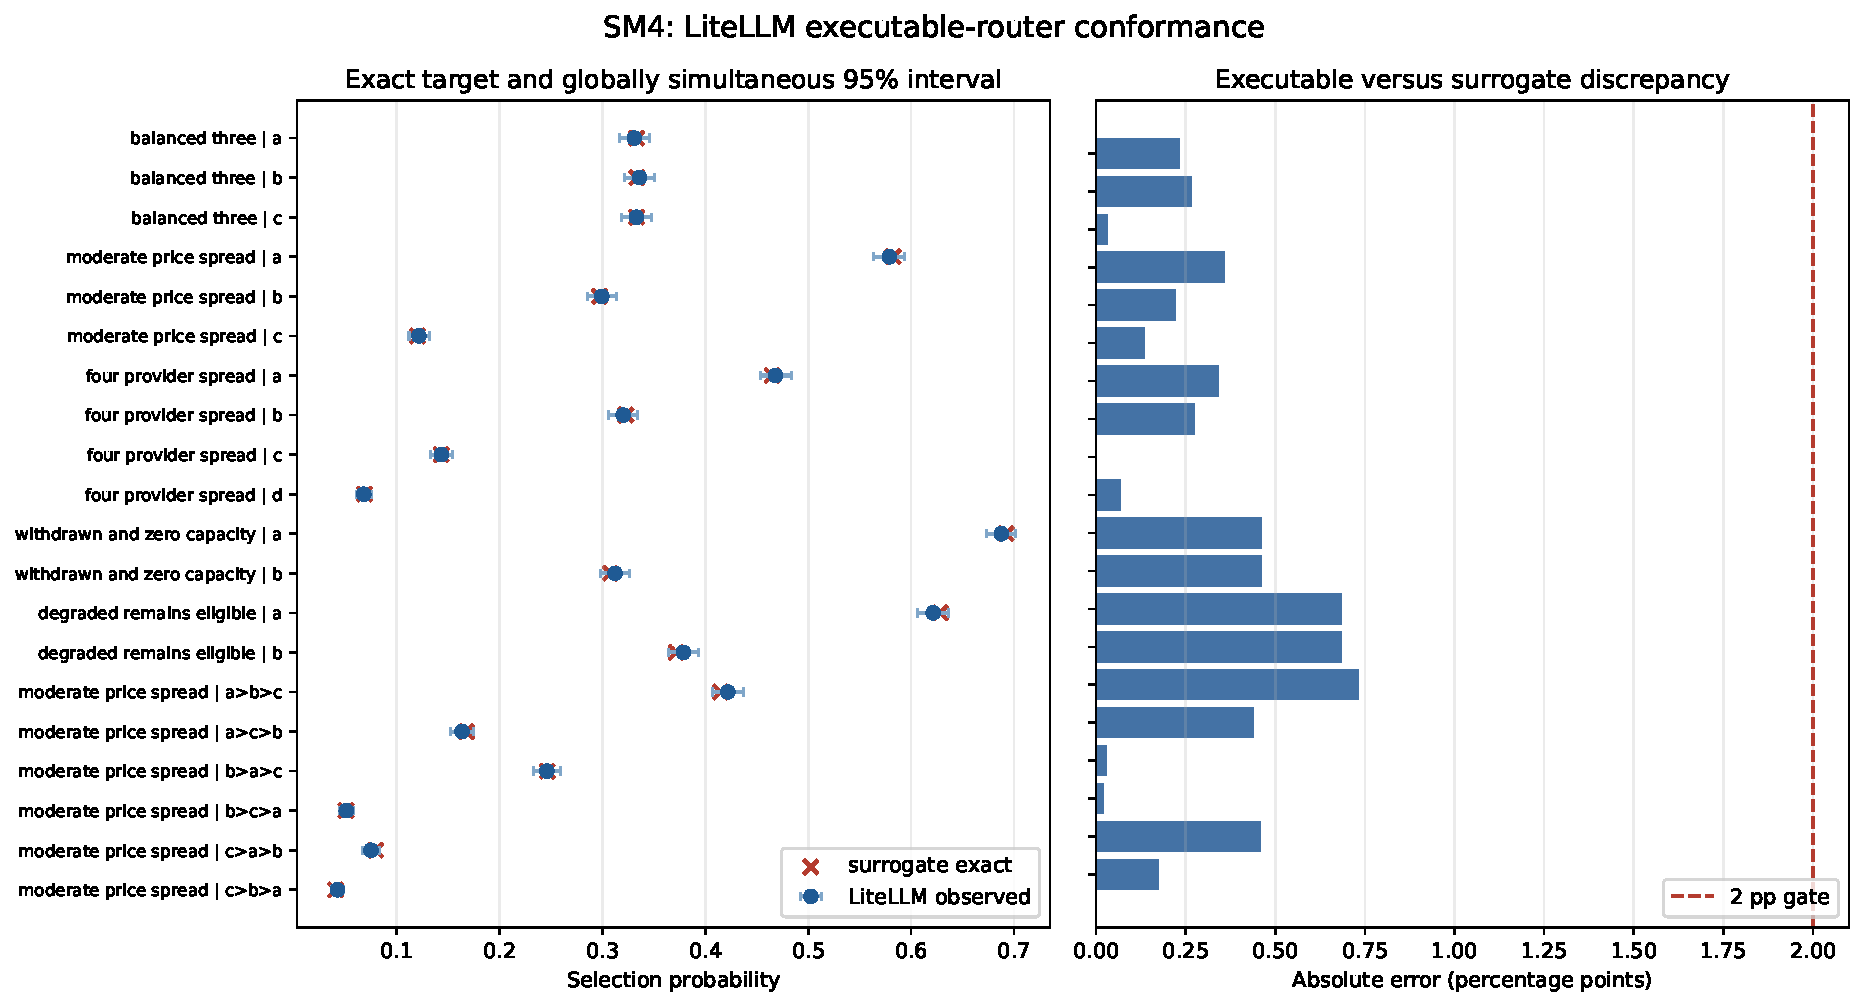
\includegraphics[width=\textwidth]{sm4_litellm_conformance.pdf}
  \caption{Executable LiteLLM conformance.  Crosses are exact surrogate
  probabilities; dots and bars are LiteLLM frequencies and globally
  simultaneous 95\% intervals.  The bottom six rows are complete fallback
  permutations, not independent first-route draws.}
  \label{fig:litellm}
\end{figure}

\FloatBarrier

\section{Results}

\subsection{Falsification: state information is not enough}

E-SIM5 enumerates all $2^7=128$ router histories.  Exact value iteration cuts
in all 20 profiles.  A Q-learner that sees only its last action stays high in
20 of 20 seeds.  Crucially, the learner that sees the complete Markov history
also stays high in 19 of 20.  Its median-price contrast relative to the aliased
learner is $-0.047$, with paired interval $[-0.142,0]$.  The registered
state-aliasing gate fails.

\subsection{Main result: temporal abstraction closes the local gap}

E-SIM6 adds a \texttt{commit-low} option equal to $M+1$ primitive low actions.
Exact primitive and option values agree over every state within $10^{-10}$.
At $M=7$, the option learner chooses the exact action and has at most 5\%
normalized regret in 18 of 20 seeds, versus 1 of 20 primitive learners.  The
option-minus-primitive regret contrast is $-0.0643$ with interval
$[-0.0755,-0.0493]$.

The memory sweep gives the mechanism check in \cref{fig:esim6}.  Both learners
succeed at $M\in\{1,3,5\}$.  At $M=7$ and $9$, exact optimization still cuts
while primitive learning usually fails.  At $M=12$, beyond the rational
boundary, exact optimization stays high; primitive learning agrees in 20 of
20 seeds, while the option overcommits and adds 0.0942 normalized regret
($[0.0735,0.1160]$).  The intervention is helpful in the delayed-credit
region, not universally.

\begin{figure}[t]
  \centering
  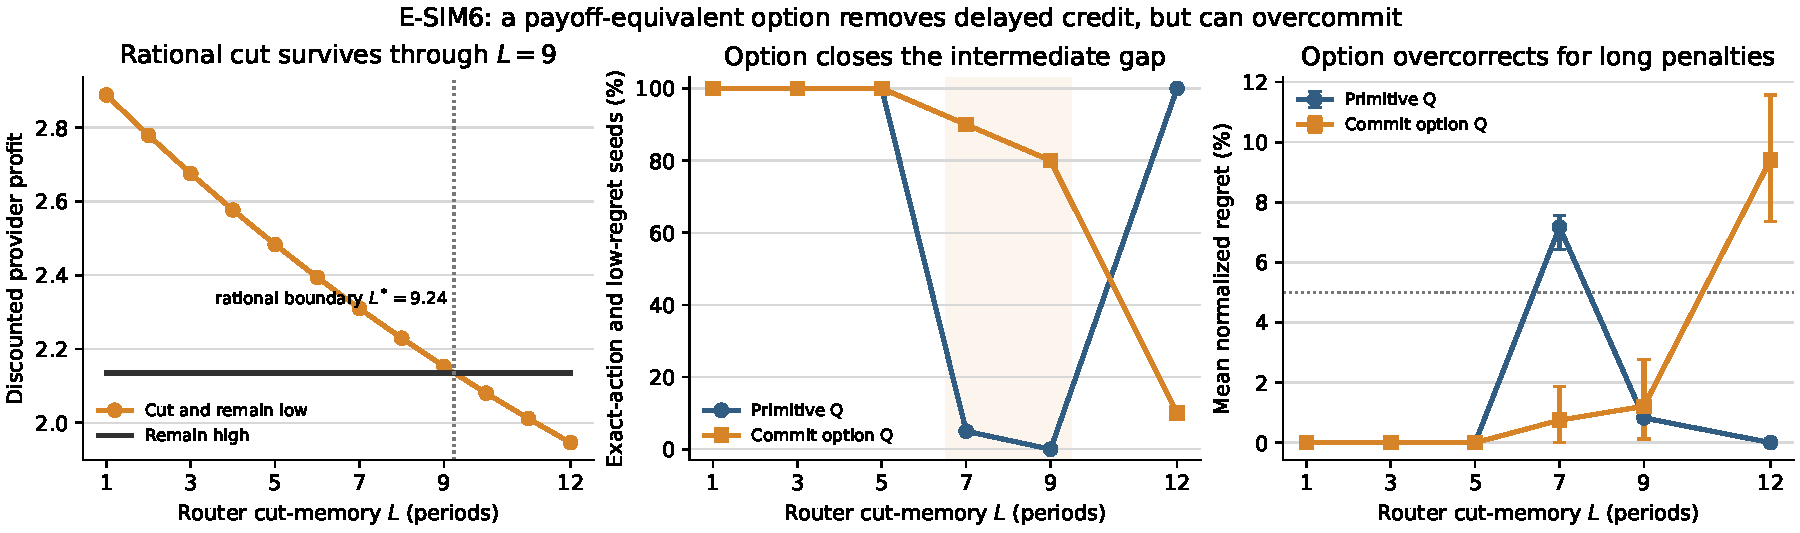
\includegraphics[width=\textwidth]{sm3_esim6_delayed_credit.pdf}
  \caption{Exact provider value, successful learning, and normalized regret
  across the router memory sweep.  The dotted boundary is derived from
  \cref{eq:boundary}; it is not fitted to the learning outcomes.}
  \label{fig:esim6}
\end{figure}

\begin{table}[t]
  \centering
  \caption{Registered E-SIM6 gates at the calibrated memory $M=7$.}
  \label{tab:gates}
  \begin{tabular}{lcc}
    \toprule
    Gate & Threshold & Result \\
    \midrule
    Exact option-value gap & $\le10^{-10}$ & pass \\
    Regret interval & upper endpoint $<0$ & pass \\
    Option exact-action/low-regret & $\ge16/20$ & $18/20$ \\
    Primitive exact-action/low-regret & $\le4/20$ & $1/20$ \\
    Composite mechanism gate & all components & pass \\
    \bottomrule
  \end{tabular}
\end{table}

\subsection{Transport and robustness}

E-SIM7 applies the same design to four frozen calibrated price books.  The
strict transport gate fails: only two markets are delayed-credit eligible,
and primitive success there is 12/20 and 14/20 rather than at most 4/20.
The prespecified rational-boundary classification nevertheless aligns with all
four effect signs.  In eligible Kimi K2.6 and GLM-5.1 books
($M^*=26.31,27.91$), the option lowers normalized regret by 0.178 and 0.118.
In ineligible GLM-5.2 and DeepSeek V4 books ($M^*=2.59,2.67$), it adds 0.155
and 0.152.  This is descriptive sign transport, not confirmation of universal
trap severity.

E-SIM8 varies learning rate
$\alpha\in\{0.05,0.15,0.30\}$ and exploration decay
$\beta\in\{1,2,4\}\times10^{-5}$.  The composite gate passes in seven of nine
cells.  All nine regret intervals are strictly negative, and option success is
18/20 or 19/20 throughout.  The failed cells have $\alpha=0.30$ and slower
exploration decay: primitive success increases, so the severity criterion
fails even though the option remains beneficial.

\begin{figure}[t]
  \centering
  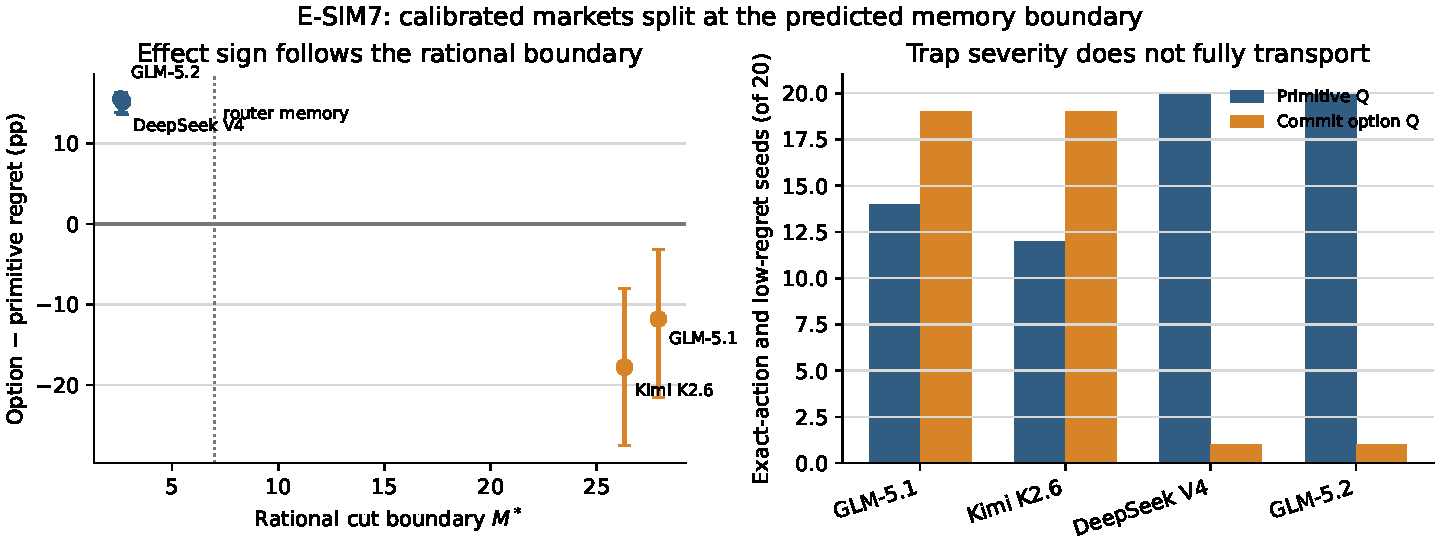
\includegraphics[width=\textwidth]{sm3_esim7_market_transport.pdf}
  \caption{Cross-market transport.  Effect signs align with the rational
  memory boundary, while the registered severe-trap gate fails.}
  \label{fig:esim7}
\end{figure}

\begin{figure}[t]
  \centering
  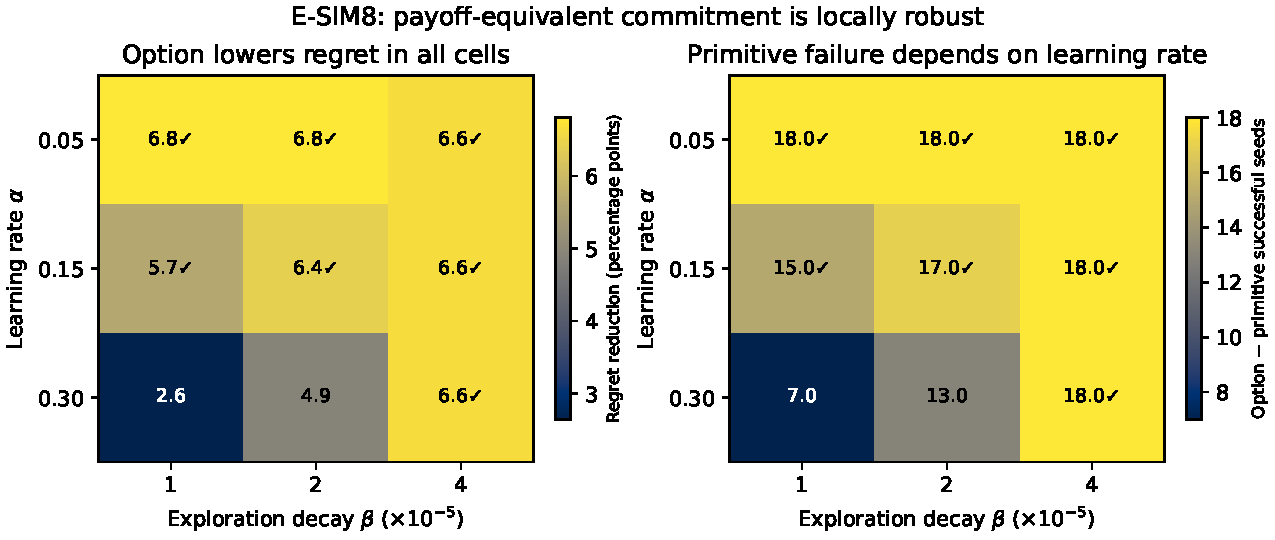
\includegraphics[width=0.86\textwidth]{sm3_esim8_q_robustness.pdf}
  \caption{Local Q-learning robustness.  Checkmarks denote cells satisfying
  the complete registered conjunction, not significance stars.}
  \label{fig:esim8}
\end{figure}

\subsection{Falsification: an ordinary multi-step target is insufficient}

E-SIM9 holds the primitive action set and every feasible price path fixed but
replaces the one-step target with an eight-step Q target spanning the complete
penalty window.  It yields 0/20 successful learners, versus 1/20 for one-step Q
and 18/20 for the option benchmark.  Its normalized-regret contrast relative
to one-step Q is $+0.0038$, with paired seed-bootstrap interval
$[0,0.0113]$.  The registered gate fails.  Thus E-SIM6 is an
option-specific temporal-abstraction result, not evidence that every longer
return operator solves the problem.

\begin{figure}[t]
  \centering
  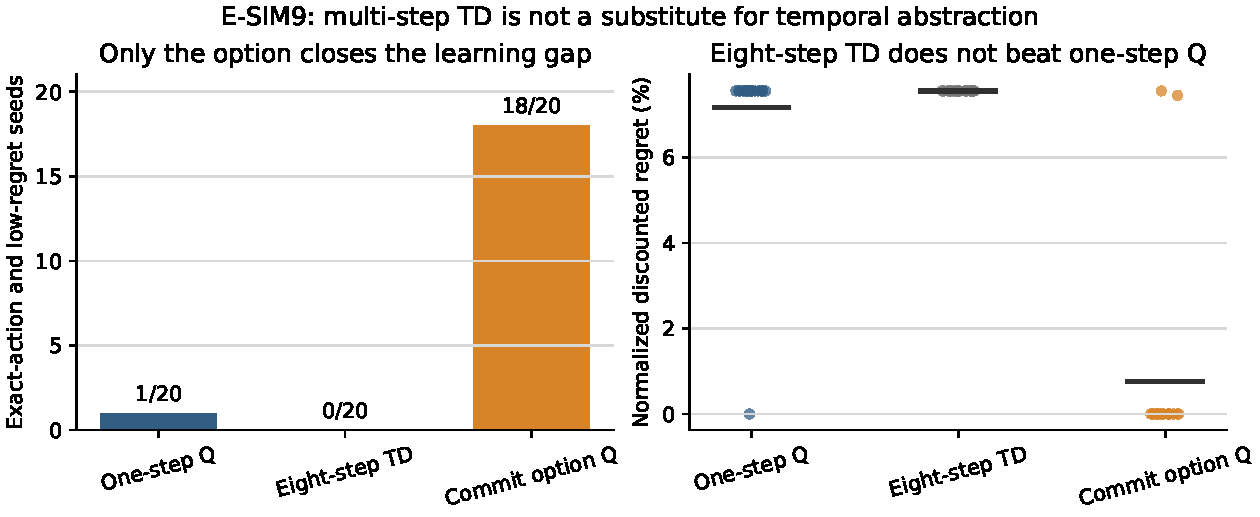
\includegraphics[width=0.86\textwidth]{sm3_esim9_multistep_falsification.pdf}
  \caption{Registered falsification.  Eight-step TD does not substitute for
  the path-equivalent commitment option.}
  \label{fig:esim9}
\end{figure}

\FloatBarrier

\section{Relation to prior work}

Inverse-power allocation is a constant-elasticity differentiated-products
demand system; variable-markup nested-CES models provide the closest static
analogy \citep{atkeson2008}.  We treat the router exponent as a public design
primitive rather than an estimated taste parameter.

Algorithmic-pricing studies show that learning protocols, timing, and platform
design can alter prices \citep{calvano2020,asker2022,brownmackay2023,johnson2023}.
\citet{brownmackay2025} derive coercion when a fast firm commits to a
multi-period rule that disciplines a rival.  Our mechanism is different: no
provider reacts to another provider's commitment rule; the router imposes an
own-cut allocation penalty, and the original high-price path is rejected as an
equilibrium.

Temporal abstraction and option Q-learning are classical
\citep{sutton1999}.  Recent work studies delayed reward and sequence
compression directly \citep{han2022,ramesh2024}.  Our contribution is not the
options framework.  It is the derivation of the delay from a marketplace rule,
the exact economic memory boundary, and the nonmonotone interaction between
that boundary and a path-equivalent learning interface.

\section{Limitations and claim boundary}

The baseline theory has captive demand, no capacity binding, and the documented
non-tool-calling price-weighted rule after eligibility filtering rather than the
proprietary implementation.  The cut multiplier is
a conditional association from one buyer tier.  Treating it as a multiplicative
weight and the trailing window as exact memory is calibration, not randomized
identification.  Costs are identified sets.

The main experiment fixes rivals and restricts the provider to the audited high
quote and best persistent cut.  It identifies a finite-MDP mechanism, not an
equilibrium of the full provider game.  Twenty seeds vary learning randomness
around one payoff profile.  E-SIM8 gives local tabular-Q robustness; E-SIM7
rejects universal severe-trap transport.  E-SIM9 shows that an ordinary
eight-step target is not a substitute for the option; other return operators
and traces remain untested.  Deep RL, LLM pricing agents, endogenous
rivals, request-serving systems fidelity, and longer calibration panels are
future tests.  LiteLLM conformance validates the mapped selection paths only;
it does not identify OpenRouter's live implementation.  No result establishes
provider intent, communication, collusion, or a
causal effect in the live router.

\section{Conclusion}

The router is the provider's demand curve, and its memory shapes which price
paths a bounded algorithm can discover.  Inverse-square allocation creates a
classical static markup floor.  The new result is dynamic: at the calibrated
seven-period cut penalty, cutting is rational but delayed credit keeps primitive
Q-learning high.  A path-equivalent commitment option closes that local gap and
then overcorrects beyond the rational boundary.  An ordinary longer TD target
does not reproduce the effect, which confines the result to this action
abstraction.  Marketplace design should
therefore evaluate both rational incentives and the learning dynamics induced by
its interfaces.

\appendix
\section{Proofs}

\begin{proof}[Proof of the share and single-crossing lemma]
Write $s_i=w_i/(w_i+W_{-i})$, where $w_i=p_i^{-a}$ and $W_{-i}$ is fixed.
Differentiation gives
$\partial s_i/\partial p_i=-(a/p_i)s_i(1-s_i)$.  Hence
\[
  \frac{\partial\pi_i}{\partial p_i}
  =Ds_i\left[1-a(1-s_i)\frac{p_i-c_i}{p_i}\right].
\]
Both $1-s_i(p_i)$ and $(p_i-c_i)/p_i$ are strictly increasing above cost.
Their product crosses one at most once, which proves quasiconcavity and the
best-response statement.
\end{proof}

\begin{proof}[Proof of \cref{thm:static}]
At symmetry $s_i=1/n$.  The interior first-order condition becomes
$a(1-1/n)(p-c)/p=1$, which yields the formula and requires
$a(n-1)>n$.  If the inequality fails, the derivative at every symmetric
interior profile is positive and the cap is the only symmetric pure-strategy
solution.
At any interior equilibrium,
$(p_i-c_i)/p_i=1/[a(1-s_i)]>1/a$, which rearranges to the markup floor.
As $s_i\to0$, the inequality converges to equality.
\end{proof}

\begin{proof}[Proof of \cref{thm:boundary}]
In the all-low state, low strictly dominates high by
\cref{eq:ordering}; a high action would also reinsert a high quote into memory.
Before the all-low state, any high action resets progress.  Any policy that
eventually cuts can therefore be weakly improved to $k$ high actions followed
by low forever.  Its value is
\[
  V_k=\frac{u_H(1-\gamma^k)}{1-\gamma}+\gamma^kV_{\mathrm{cut}},
  \quad
  V_{\mathrm{cut}}=
  \frac{(1-\gamma^M)u_{\theta L}+\gamma^Mu_L}{1-\gamma}.
\]
Since $V_k-u_H/(1-\gamma)=\gamma^k[V_{\mathrm{cut}}-u_H/(1-\gamma)]$,
either $k=0$ or never cutting is optimal.  Comparing these alternatives and
rearranging gives \cref{eq:boundary}.
\end{proof}

\begin{proof}[Proof of \cref{thm:option}]
The augmented action set contains all primitive actions, so its optimal value is
weakly larger.  Conversely, replace every option in any augmented policy by its
finite defining sequence of primitive actions.  The unrolled policy is feasible
in the primitive MDP and produces the same states and discounted rewards.  Its
value is therefore identical, so the augmented optimum cannot be larger.
\end{proof}

\section{Reproducibility}

The clean confirmatory bundles are E-SIM5 \texttt{3e5a55405e}, E-SIM6
\texttt{93265b9b03}, E-SIM7 \texttt{bd74ab2eb7}, and E-SIM8
\texttt{4d84b9b3a2}; the registered E-SIM9 falsification is
\texttt{179eca0f9d}.  Every manifest records source commit
\texttt{4f9007b}, a result hash, input-artifact hashes, and equality between the
executed market-environment source and the source stored at that commit.  Exact
Bellman residuals, option-value equality, and paper-number crosswalks are
enforced by the test suite.  The LiteLLM conformance release executes from
source commit \texttt{1e62de3}; its manifest pins LiteLLM 1.92.0, hashes both
executed selector functions, and hashes every table, figure, and report.

\bibliographystyle{plainnat}
\bibliography{references}

\end{document}
